
The experiments will run the \rrtfunnel{} against a benchmark regular RRT
planner with the motion primitive set pictured
in \cref{fig:intial-trajectories-exp} on a forest traversal problem. The
benchmark-planner is a RRT algorithm employing the same motion primitive set as
the \rrtfunnel{} algorithm, with the same LQR controller, and the same distance
metric. The difference is that the benchmark planner does not take uncertainty
into account, and instead maximizes the distance to the nearest obstacle as the
extension operator i.e.,
\begin{equation}
  \max_{i}\min_{t,j} \bigl( \vect{x}_{i}(t), o_{j} \bigr)
\end{equation}
where \(x_{i}(t) \in \mathcal{T}\), is a trajectory from the basic motion
primitive set, and \(o_{j} \in \modelobstacle{}\) is an obstacle in the
configuration space \(\modelconfigurationspace{}\). Note also that in order to
guide the expansion towards the goal, a goal bias of \(10\%\) is given to the
benchmark planner, which is beneficial for decreasing the dispersion of the
algorithm~\cite{Lav06}. This is introduced to counter the distance metric, which
tries to maximize the distance to the obstacles.

The end goal is set so that it will not take pose into account, and will only be
concerned with getting within an \(\epsilon\) of the \((x,y)\) in the test map.
For all the experiments an \(\epsilon\) of 5\IEEEunit{m} is given to the
planners.

Each test-run will be run in a forest generated with a \textit{Poisson process}
method.

The experiments will record the number of collisions for each algorithm across
all test-runs. The planners will run in the same environment for each test, with
the same initial starting point. The environment will be redrawn using the Poisson process to generate the obstacle forest for each consecutive run.
With this test setup the difference between the planners should become evident.

Before the experiments are run, all individual funnels in the base set are run
with a hundred simulations runs from random starting positions in its inlet, to
check if the invariant holds, and that the model stays within the funnel at all
times. Uncertainty is added in terms of an additive noise with \(w =
0.3\) \IEEEunit{m/s} in the world \(x\)-direction, imitating a cross-wind.

\subsection{Experiment Setup}

The algorithm will be tested by generating a random strip of forest of depth
\(25\)\IEEEunit{m}, and then letting the \rrtfunnel{}, along with the benchmark algorithm
find a way through the environment to the other side. Three seperate experiments will be conducted where the amount of crosswind will vary. The first experiment will have a crosswind of \(0\) \IEEEunit{m/s}, in order to set up
the experiment baseline. The second experiment will have a crosswind of \(0.3\) \IEEEunit{m/s},
which is the maximum crosswind modelled in the \rrtfunnel{} algorithm. This experiment will
show the difference between explicitly handling uncertainty in comparison to
handling it heuristically. Lastly, an experiment with a \(0.6\) \IEEEunit{m/s} is perfomed, to
verify the assumed result that if the uncertainty assumptions are broken the \rrtfunnel{} algorithm
does no longer guarantee safe traversal.

The obstacles are imagined to be trees
with trunks modelled as circles with a radius of \(0.1\) \IEEEunit{m}, and are
placed randomly on the area \(O=\{ \vect{x} \mid -50 \le x_{1} \le 50 \text{ and
} 5 \le x_{2} \le 25 \}\), as the realization of a \textit{Poisson process} with
density
\(\lambda = 0.2\). For each trial run, a new forest is generated in
this random fashion, and the algorithms are given the task to traverse the
generated map in turn, see~\cite{Kroese_2014} for an introduction to Poisson
processes.

The funnels for the \rrtfunnel{} algorithm are in this case made to handle
uncertainty, in the form of a cross-wind up to and including \(3\)
\IEEEunit{m/s} in the x-direction of the airplane, but does not currently have
any control over the y-direcction. Since the model used is single input, and
only controls the angle of travel, not the speed of the aircraft.
A maximum of \(5000\) nodes is set as an upper treshold on both of the algorithms'
exploration trees.

\subsection{Generating Robust Motion Primitives}

This paper employs the simple unicycle model from
\author{Lav06}~\cite{Lav06} which is modified slightly into
\begin{equation}
  \label{eq:model-dynamics} \vect{x} = \begin{bmatrix} x \\
  y \\ \theta \\ \end{bmatrix}, \, \dot{\vect{x}} = \begin{bmatrix}
  -v \sin(\theta) \\ v \cos(\theta) \\ u \\ \end{bmatrix} ,
\end{equation}
which is a first-order unicycle model with a constant speed. Although this is
the only model used in this paper, the method can be adapted
into accommodating a different and more complex model.


%\subsubsection{Generating the Trajectories}

The trajectories for the base set of motion primitives is generated through the
direct collocation method on the dynamical system given in
\eqref{eq:model-dynamics}.

The basis set of motion primitives should be small, yet cover enough of the
finer movements of the dynamical system so that the motion of the planning unit
can be near continuous when composed together. Thus in order to generate a dense
set of motion primitives, points along the arc of a circle with \(N\)
different radii as the initial points for the trajectory generator described in
\cref{subsec:generating-the-trajectories}. The initial trajectories employed in
the experiments can be seen in \cref{fig:intial-trajectories-exp}.

\begin{figure}[!t]
  \centering
  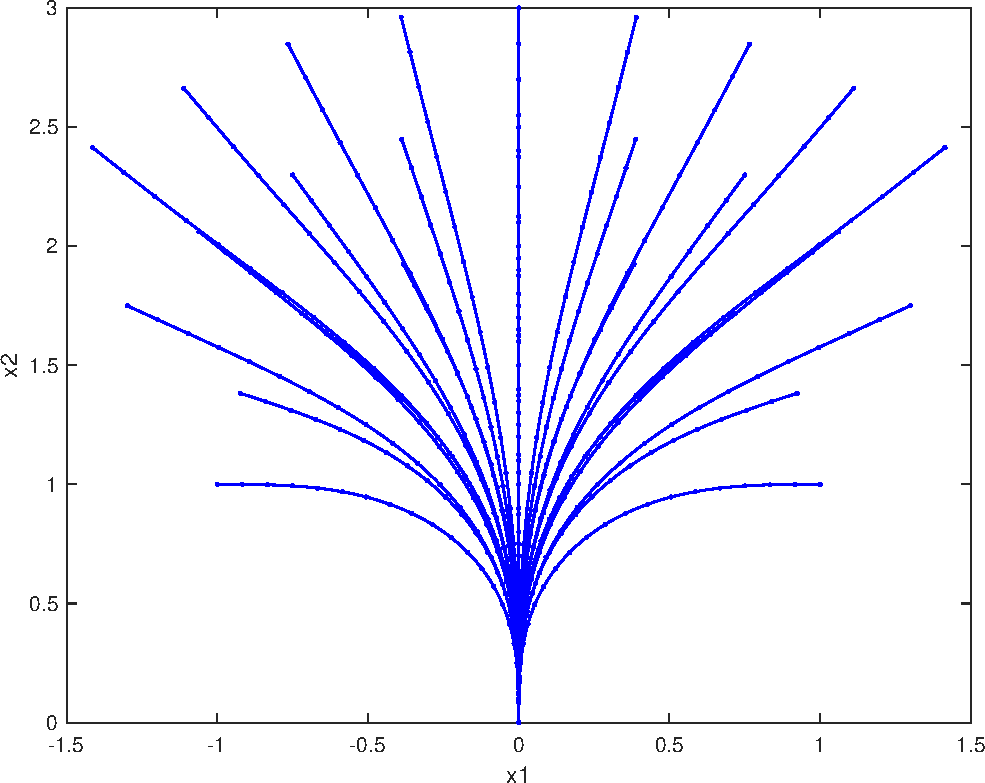
\includegraphics[width=.8\columnwidth]{figures/experiments/initial-trajectories}
  \caption[The experiment trajectory set]{The initial trajectories used in the
    \rrtfunnel{} algorithm.}
  \label{fig:intial-trajectories-exp}
\end{figure}



\subsection{Initializing the Funnel Calculations}

As noted in \cref{subsec:initializing-tvlqr}, the funnel calculations need to be
initialized with a candidate Lyapunov function. For this paper, this is a TV-LQR controller.

Then to get the initial Lyapunov function, the system error dynamics are
linearized.
\begin{equation}
  \dot{\bar{\vect{x}}} \approx \matr{A} (t)\bar{\vect{x}}(t) + \matr{B}(t) \bar{\vect{u}}(t)
\end{equation}
\begin{equation}
  \dot{\bar{\vect{x}}} \approx %
  \begin{bmatrix}
    0 & 0 & -v\cos(\theta) \\
    0 & 0 & -v\sin(\theta) \\
    0 & 0 & 0 \\
  \end{bmatrix} %
  \bar{\vect{x}} (t) %
  + %
  \begin{bmatrix}
    0 \\ 0 \\ 1
  \end{bmatrix} %
  \bar{\vect{u}}(t),
\end{equation} 
which is an an initial candidate Lyapunov function of the form
\begin{equation}
  V(t,\bar{\vect{x}}) = {\bar{\vect{x}}}^{T} \matr{S}_{i}\bar{\vect{x}} ,
\end{equation}
where \(S_{i}\) is a solution of the \textit{Ricatti} equation
\begin{IEEEeqnarray*}{Cr}
  \label{eq:ricatti}
  - \dot{\matr{S}}(t) = \matr{A}^{T} \matr{S}(t) +\matr{S}(t) \matr{A} - \left( \matr{S}(t) \matr{B} + \matr{N} \right) \matr{R}^{-1} \IEEEyesnumber \\
  \IEEEeqnarraymulticol{2}{r}{\left( \matr{B}^{T} \matr{S}(t) + \matr{N}^{T} \right) + \matr{Q}}
\end{IEEEeqnarray*} 
associated with the LQR controller. The feedback is gained from
\[
  \matr{K}(t) = \matr{R}^{-1} \left( \matr{B} \matr{S}(t) + \matr{N}^T \right),
\]
and enables the system dynamics \cref{eq:model-dynamics} to be written
\(f_{\mathit{cl}}(t,\vect{x})\) by direct substitution of \(\vect{u} =
-K\vect{x}\), where \(K\) is a \(1 \times 3\) matrix, and hence making the system in \cref{eq:model-dynamics} 
dependent only on \(t\) and \(\vect{x}\),
\begin{equation}
  \label{eq:model-dynamics-cl}
  \vect{x} =
  \begin{bmatrix}
    x \\ y \\ \theta \\
  \end{bmatrix}, \, \dot{\vect{x}} =
  \begin{bmatrix}
    -v \sin(\theta) \\
    v \cos(\theta) \\
    -K\vect{x} \\
  \end{bmatrix} \mathEoS
\end{equation}

Which means that

\[
V_{i}(t, \vect{x}) = \vect{x}^{T}S_{i}\vect{x}
\]
as needed.

\kma{Kom hit}

\subsection{Generating the Funnels around the Initial Trajectories}

With the inital trajectory set defined, it is time to generate the funnels
around them, so that safe traversal can be guaranteed. Thus for this to happen,
the funnel generator needs an initial condition set from which to start. This is
given by the hyper-ellipsoid
\begin{align}
  \mathcal{X}_0 &= \set{\vect{x} \in \R^{3} \mid \vect{x}^{T} Q \vect{x}} \\
  Q &= \begin{bmatrix}
    2 & 0 & 0 \\
    0 & 2 & 0 \\
    0 & 0 & 4
  \end{bmatrix} \mathEoS
\end{align}
which means that the dynamical system can start in a wide variety of initial
states, and the controller will be able to take it safely to the outlet of the
funnel. This is also beneficial, as this means it is easier to compose with
another funnel, as the inlet is bigger.

\subsection{Funnel Transformation and Invariance}

Given the model from \cref{eq:model-dynamics} the cyclic coordinates of the
system are found from:
\begin{align*}
  \mathcal{L} &= T - V = \frac{1}{2} mv^2 + \frac{1}{2}I\dot{\theta}^2 \\ 
              &= \frac{1}{2} \left(  m \left(
                \dot{\vect{x}}^2 \sin^2 \theta + \dot{\vect{x}}^2 \cos^2 \theta
                \right)  + I {\dot{\theta}}^2 \right) \\
              &= \frac{1}{2} \left(  m\dot{\vect{x}}^2 + I {\dot{\theta}}^2 \right)
\end{align*}
which shows that the Lagrangian is invariant to shifts in the \((x,y,\theta)\)
variables, since \(\frac{\partial\mathcal{L}}{\partial q_i} = 0, \, q_i =
x,y,\theta\). Now any funnel in the base set can be shifted freely around in the
cyclic coordinates of the system without changing the solution to the system
dynamic equation, and thus create an infinite set of funnels in the state space
for the planner to work with. Through the partitioning of coordinates into
cyclic- and non-cyclic coordinates of the form \(\vect{x} = \left[ x_c\; x_{nc}
\right]^{T }\), the state dynamics \cref{eq:model-dynamics} only depends on the
cyclic coordinates of the system. Thus, a trajectory of the form \(t \rightarrow
\bigl( \vect{x}(t), \vect{u}(t) \bigr) \) which solves \(\dot{\vect{x}} = f
\bigl(\vect{x}(t), \vect{u}(t) \bigl) \) can then be transformed through a shift
\(\Psi_{c}\) along the cyclic coordinates of the system to yield a valid
solution of the form
\[
  t \rightarrow \bigl( \Psi_{x}(\vect{x}(t)), \vect{u}(t) \bigr)
\]
where the transform \(\Psi\) is given by
\[
  \Psi \bigl( \begin{bmatrix}
    \vect{x}_{c}  \\ \vect{x}_{\mathit{nc}} 
  \end{bmatrix}
  \bigr) =
  \begin{cases}
    \vect{x}_{c} \rightarrow \vect{x}^{'}_{c} \\
    \vect{x}_{\mathit{nc}} \rightarrow \vect{x}_{\mathit{nc}} \mathEoS
  \end{cases}
\]
However, since \( \dim (\vect{x}) = \dim(\vect{x}_{c}) \), for
the~\cref{eq:model-dynamics}, it is not necessary to handle the non-cyclic case.


\subsection{Funnel Composition}
\label{subsec:funnel-no-composable}

In accordance with \cref{sec:composable-funnels}, the funnel robustness
guarantees are only valid if the funnels are composable 
\cref{def:funnel-composition}. Unfortunately, the funnels do not
compose as per this definition in the experiments run, and the composition
testing of the algorithm has to be left out. Thus the experiments are run with a
funnel graph that is complete, and all funnels can compose with each other, at
the cost of the mathematical robustness guarantees of the system. This is
because the one dimensional controller employed has no influence on the speed of
the airplane, and hence there is no way to make the system converge in the
direction of speed. This is exemplified in \cref{fig:funnel-inlet-outlet}, where
the inlet is overlaid the outlets for the projected xy-funnel, and it can be
seen that the controller is able to converge the xy-funnel in the x-direction,
but not in the y-direction, as it has no control over this dimension at all. The
framework can be expanded with this functionality however, but this will be
referred to as future work.

\begin{figure}[!t]
  \centering
  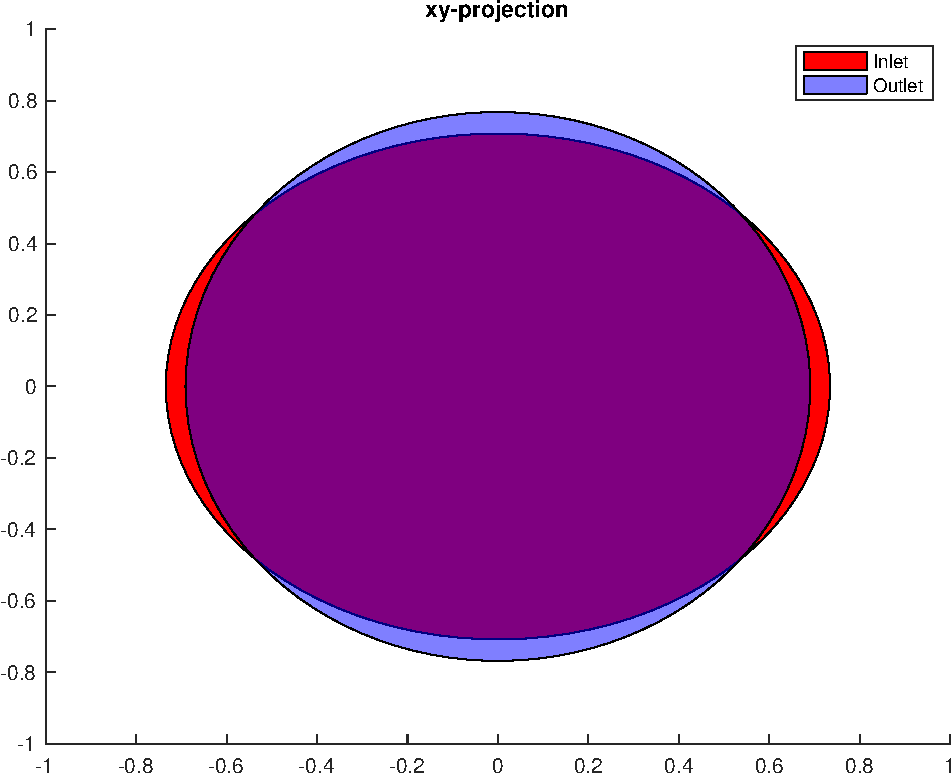
\includegraphics[width=.8\columnwidth]{figures/experiments/funnel-inlet-outlet}
  \caption[The projection of the funnel inlet and outlet in the xy-plane]{The projection of the funnel inlet and outlet in the xy-plane. It is
    seen that the controller is able to make the funnel converge in the
    x-direction as expected, however, it has no control in the y-direction, as
    there is no controller steering the speed of the vehicle.}
  \label{fig:funnel-inlet-outlet}
\end{figure}

\subsection{Continuous Verification of Invariance}
\label{subsec:check-vehicle-in-funnel}

In order to remedy this off-line compositional robustness guarantees, the
\rrtfunnel{} algorithm will keep track of whether the model has left the funnel
during execution, and aborts the simulation with the emergency maneuver if the
airplane leaves one of the funnels at runtime. This happens if the value of the
Lyapunov function is larger than one. This will be counted in the experiments as
a collision on the part of the \rrtfunnel{} algorithm. A plot of the Lyapunov
values for a simulation run can be seen in \cref{fig:lyapunov-values}.

\begin{figure}[!t]
  \centering
  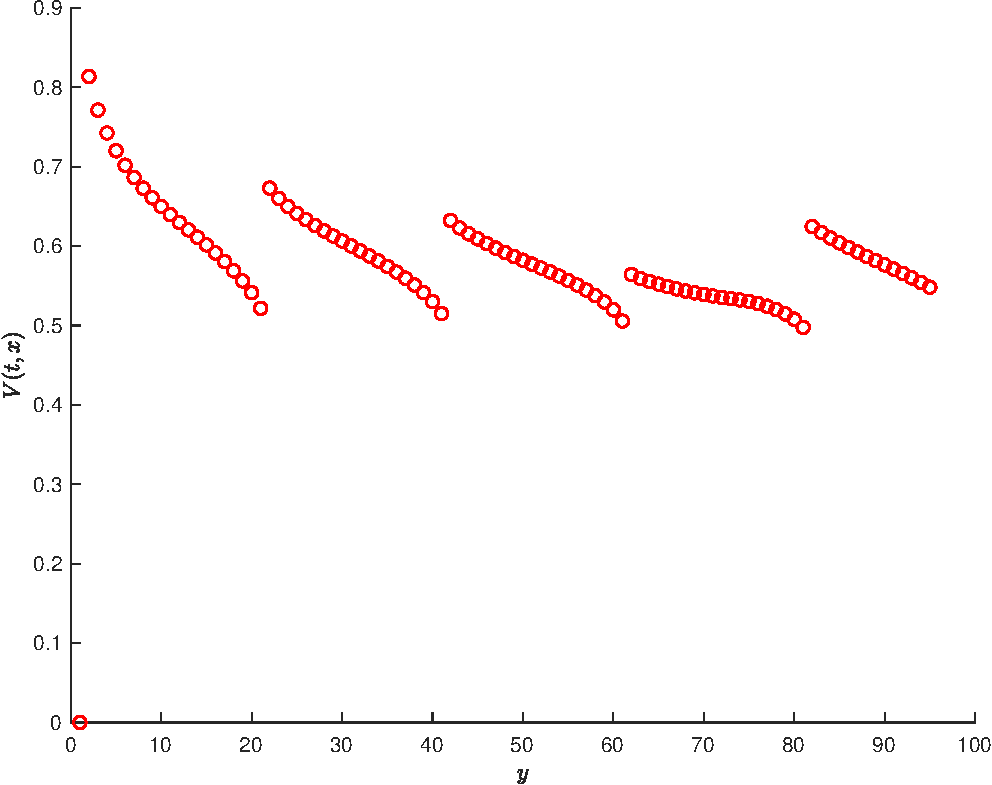
\includegraphics[width=.8\columnwidth]{figures/experiments/lyapunov-values-simulation-run}
  \caption[A plot of the Lyapunov values for an experiment]{The plot of the Lyapunov values for a simulation run at the sampling
    times \(t_k\).}
  \label{fig:lyapunov-values}
\end{figure}


\subsection{The Size of the Airplane and the Obstacles Models}
\label{subsec:deciding-model-size}

The funnels generated thus far are created from a point model of the airplane,
and its dynamics. If the grid that the simulations are run on are set to have an
unit size of one meter, then the funnels from the basic set are given a velocity
of \( [v(t)] = \text{\IEEEunit{m/s}} \), \( [\theta] = \text{\IEEEunit{rad}} \),
and \( [\dot{\theta}] = \text{\IEEEunit{rad/s}} \), where \( [\, \cdot \,] \) is
the unit operator. The size of the airplane is arbitrary, and can be chosen
freely, but if it is imagined as a radio controlled aircraft, with a speed of
\(10\) \IEEEunit{m/s}, then a size of \(10 \times 20 \) \IEEEunit{c/m} keeps
everything within the realm of a normal radio controlled aircraft and its
capabilities. The mass is not relevant for our first order dynamics, but still
the airplane is assigned a mass of \(1\, \textit{kilo}\), so that the
translation of the model dynamics is not irrelevant.

\subsection{Expanding the Funnels around the Airplane Model}
\label{subsec:expand-funnel}

The size of the airplane in the original model is a single point, and as such,
the expanded airplane model is not accounted for in the current funnels.
Therefore the funnels have to be expanded in order for them to accommodate the
necessary robustness guarantees that are expected from the algorithm. However,
the size of the airplane only affects the size of the funnel ellipsis projected
down into the xy-plane. Therefore, first extract the projected size of the
funnel, through a projection map: \(P \colon \R^4 \rightarrow \R^2\), where \(P
= \begin{bmatrix} I_{2 \times 2} & {0}_{2 \times 2} \\ \end{bmatrix} \) such
that for the projected ellipsoid
\(
  \mathcal{E}_{p} = \set{\bar{\vect{x}} \in \R^{2} \mid
    {\bar{\vect{x}}}^{T}S_{k}^{(p)}\bar{\vect{x}} \leq 1},
\)
with \(S_{k}^{(p)}\) given by
\(
  S_{k}^{(p)} = {\left( PS_{k}^{-1}P^T \right)}^{-1},
\)
is the set containing the funnel projected down into the xy-plane. Here
\(\mathcal{E}_{p}\) is the projected set of the ellipsoid in the xy-plane. In general an ellipse centered at
the origin is a linear transformation of the unit circle~\cite{lay2005linear}.
Exploiting this fact, the funnel ellipsoids can be expanded to encompass the
airplane model. Take note that the matrix \(S_{k}\) is
\textit{Positive semidefinite}, and hence can be Cholezky
factorized~\cite{lay2005linear}. Then expanded ellipsis (which now contains all
the possible states of the airplane model) is given by:
\begin{align*}
  S_{k}^{(\mathcal{P})} &= R^{T}R \\
  \vect{x} &= R^{-1}\vect{y} \\
  \mathcal{C} &= \set{\vect{y} \in \R^2 \mid \vect{y}^{T}\vect{y} \leq 1 + r_{a}} \\
  \mathcal{E}_{\mathit{exp}} &= \set{R^{-1}\vect{y} \mid \vect{y} \in \mathcal{C}} \\
\end{align*}
where \(\mathcal{E}_{\mathit{exp}}\) are the ellipsoids which contains the
volume of the airplane for all verified states in the funnel, and
\(r_{\mathit{a}}\) is the widest part of the model at hand, which in this case
is the wingspan. A picture of the initial funnel and the funnel expanded around
the airplane model can be seen in
figure~\cref{fig:expanded-funnel}.


\begin{figure}[!t]
  \centering
  %% \begin{minipage}[c]{.9\columnwidth}
  %% 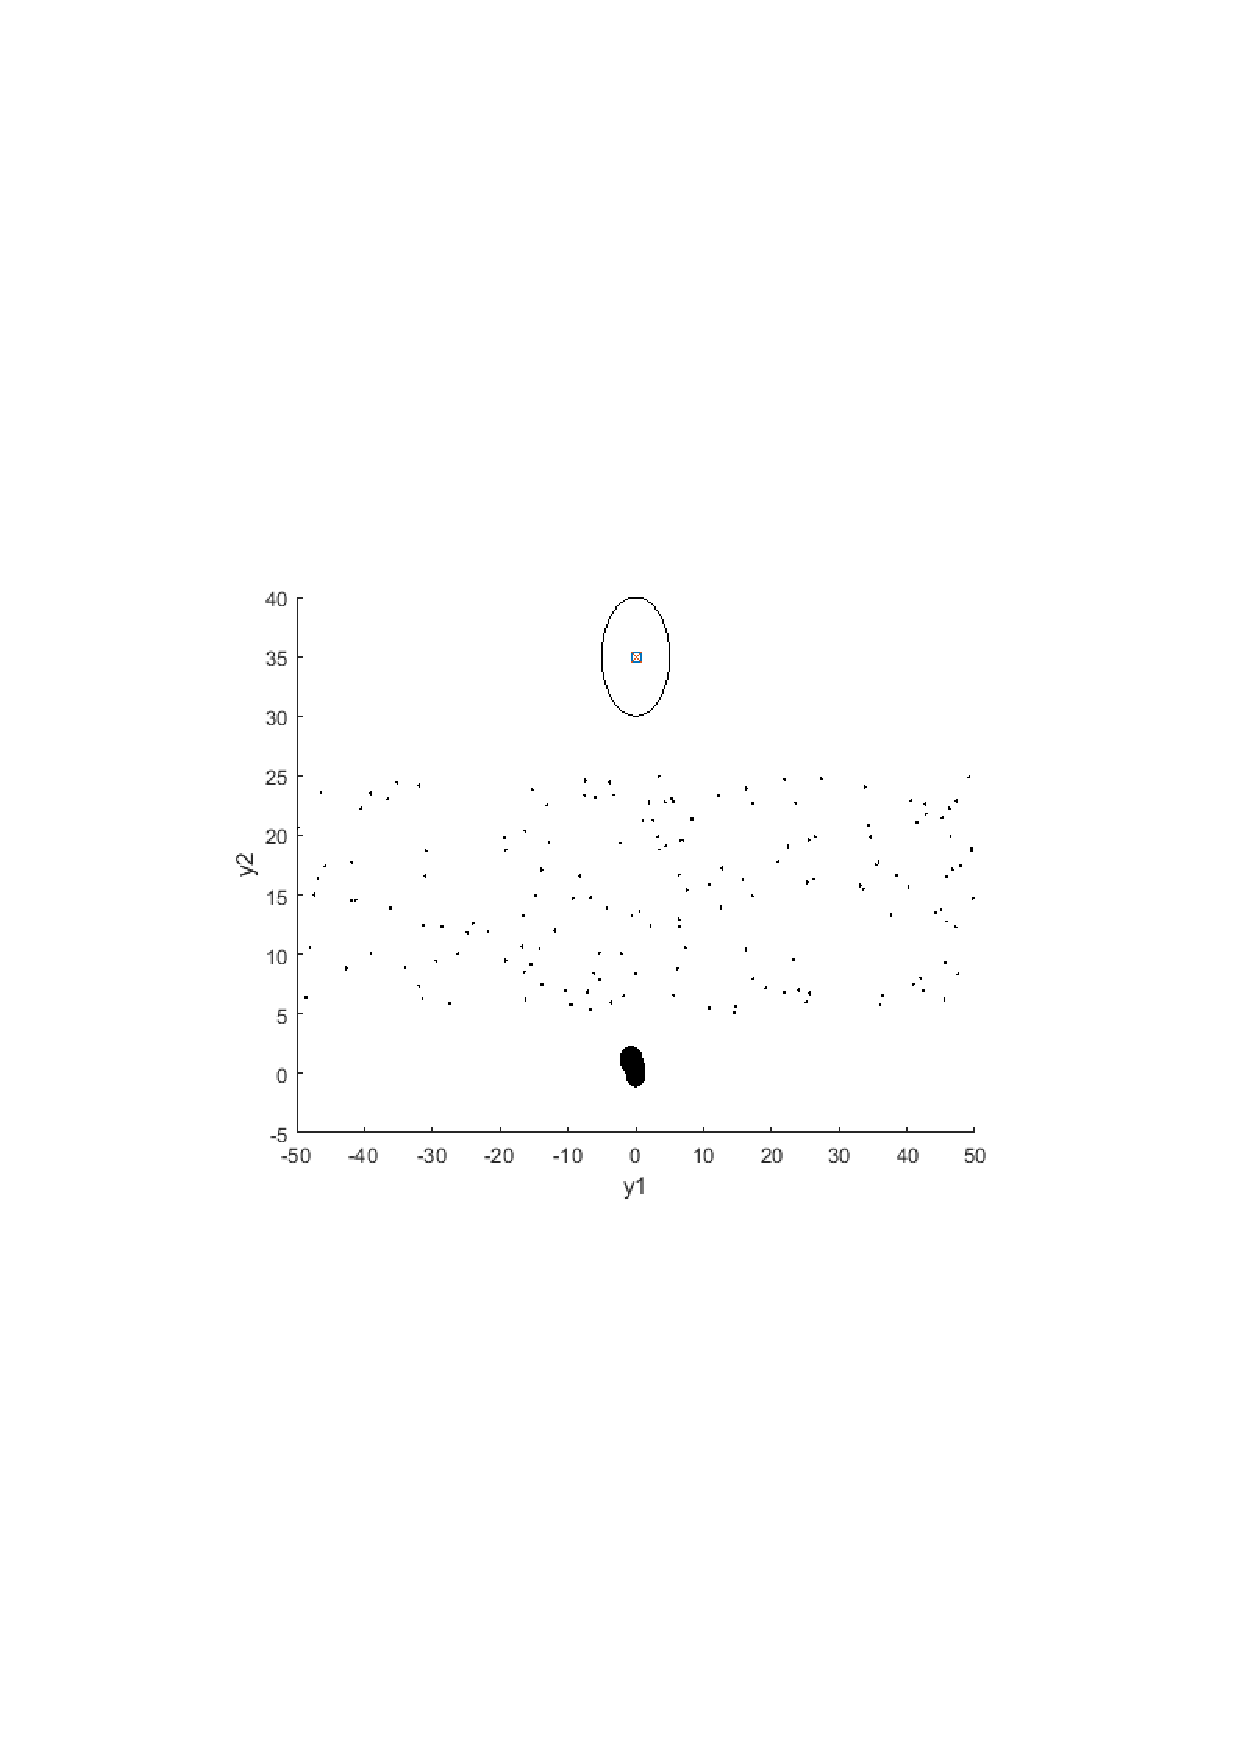
\includegraphics[scale=.5, trim={5cm, 9cm, 5cm, 7cm}, clip]{figures/experiments/rrtfunnel-1samples.pdf}
  %% \caption[The expansion of the \rrtfunnel algorithm at 1, and 101 iterations]{Visualized is the expansion of the \rrtfunnel algorithm at 1 iterations of the algorithm.}
  %% \end{minipage}
  %% \newline
  \begin{minipage}[c]{.9\columnwidth}
  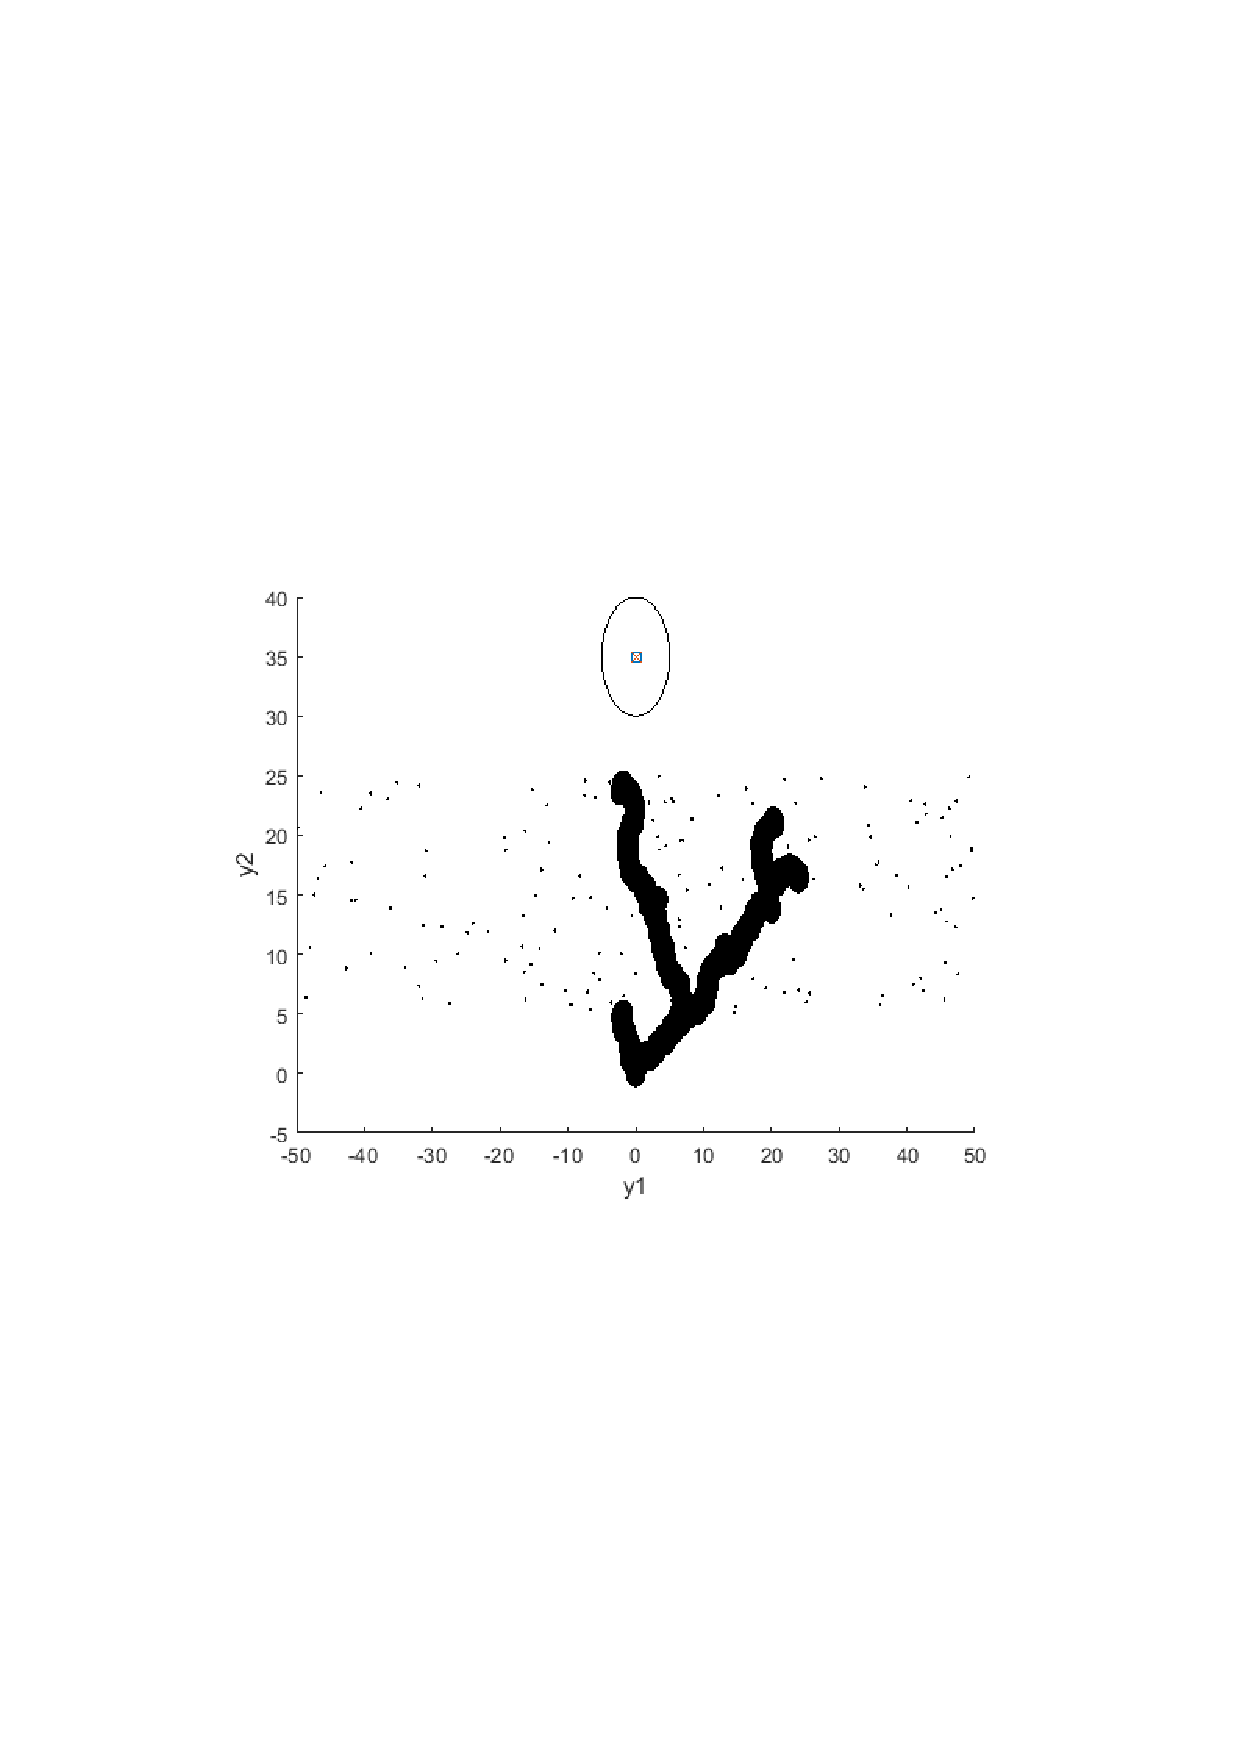
\includegraphics[scale=.5, trim={5cm, 9cm, 5cm, 7cm}, clip]{figures/experiments/rrtfunnel-101samples.pdf}
  \caption[The expansion of the \rrtfunnel algorithm at 1, and 101 iterations]{Visualized is the expansion of the \rrtfunnel algorithm at 101 iterations of the algorithm.}
  \end{minipage}
  \newline
  \begin{minipage}[c]{.9\columnwidth}
    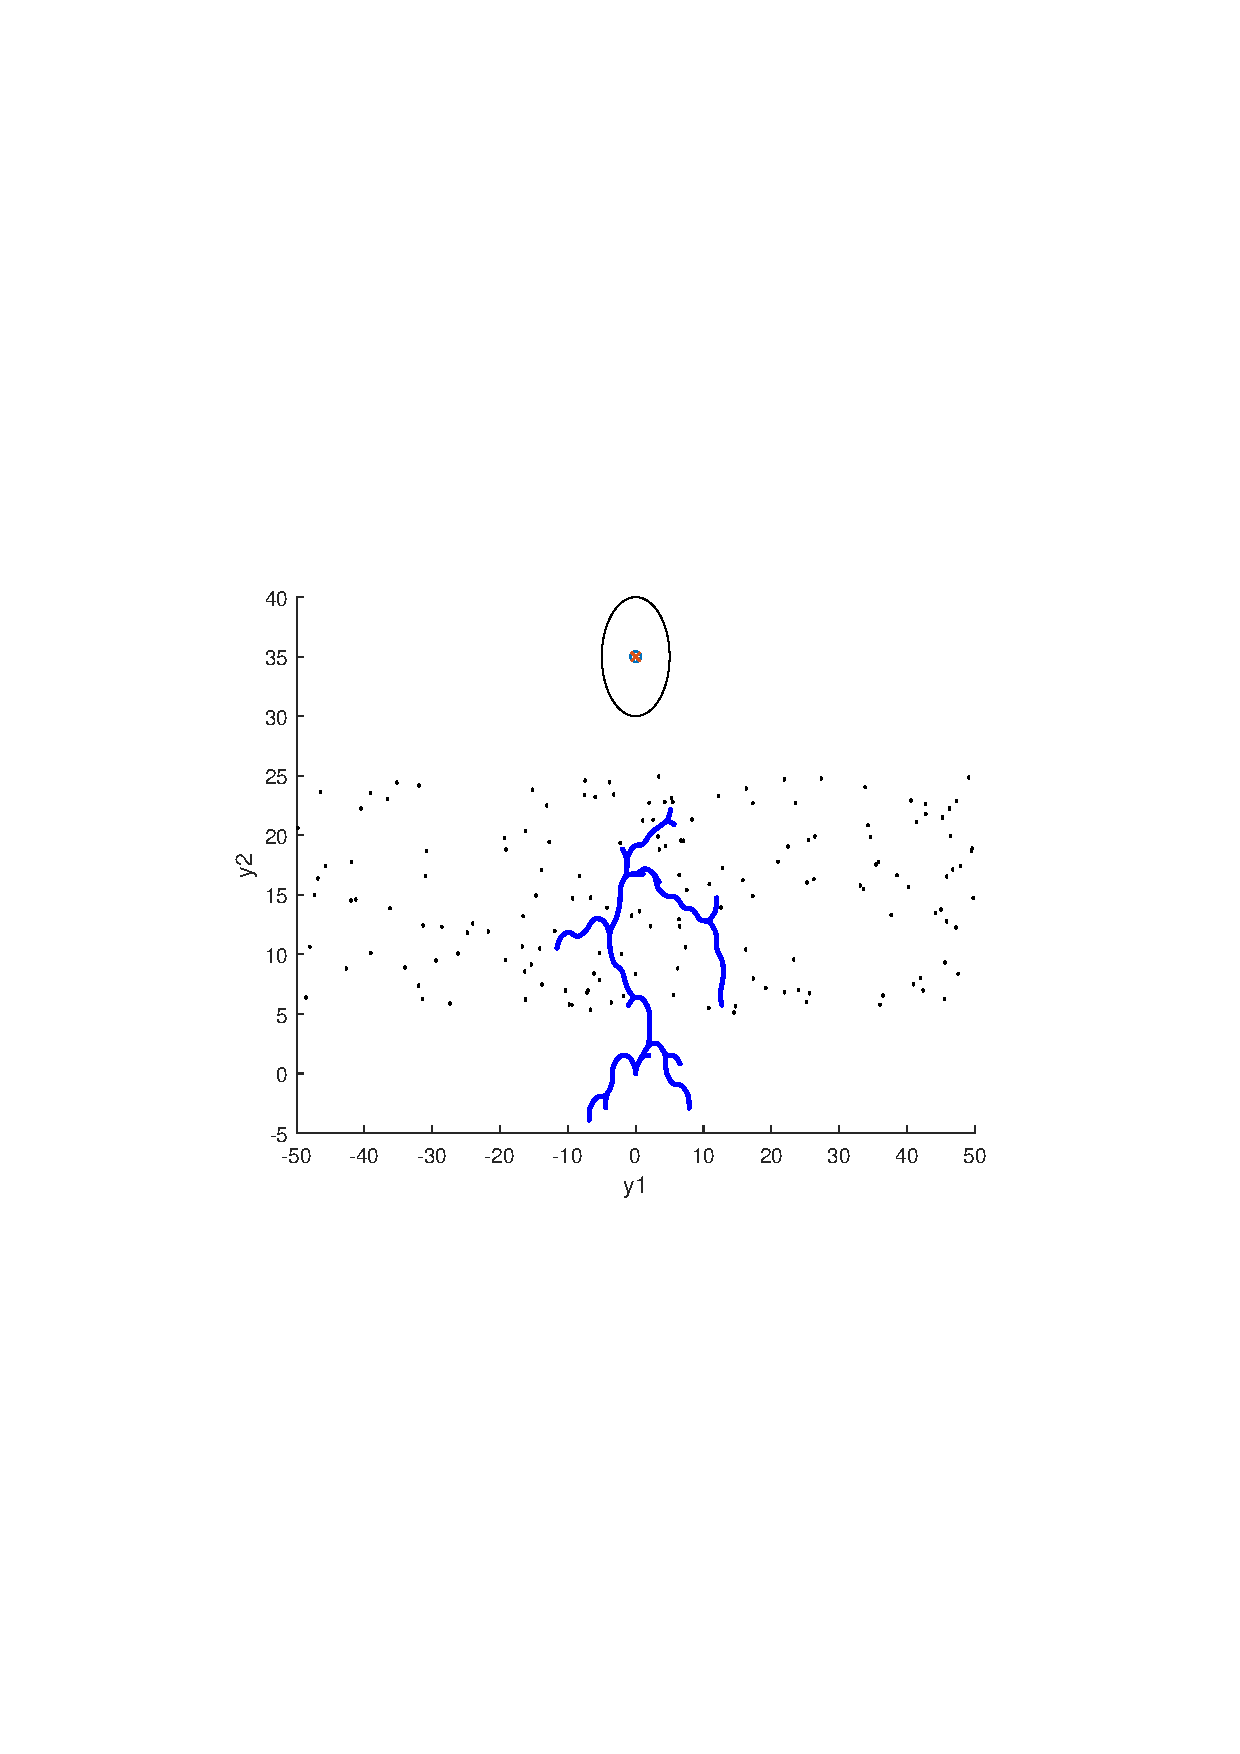
\includegraphics[scale=.5, trim={5cm, 9cm, 5cm, 7cm}, clip]{figures/experiments/rrtfunnel-101samples-dyn.pdf}
  \caption[The expansion of the \rrtfunnel algorithm at 1, and 101 iterations]{Visualized is the expansion of the \rrtfunnel algorithm at 101 iterations of the algorithm}
  \end{minipage}
\end{figure}

%% \begin{figure}[!t]
%%   \centering
%%   \begin{minipage}[c]{.8\columnwidth}
%%   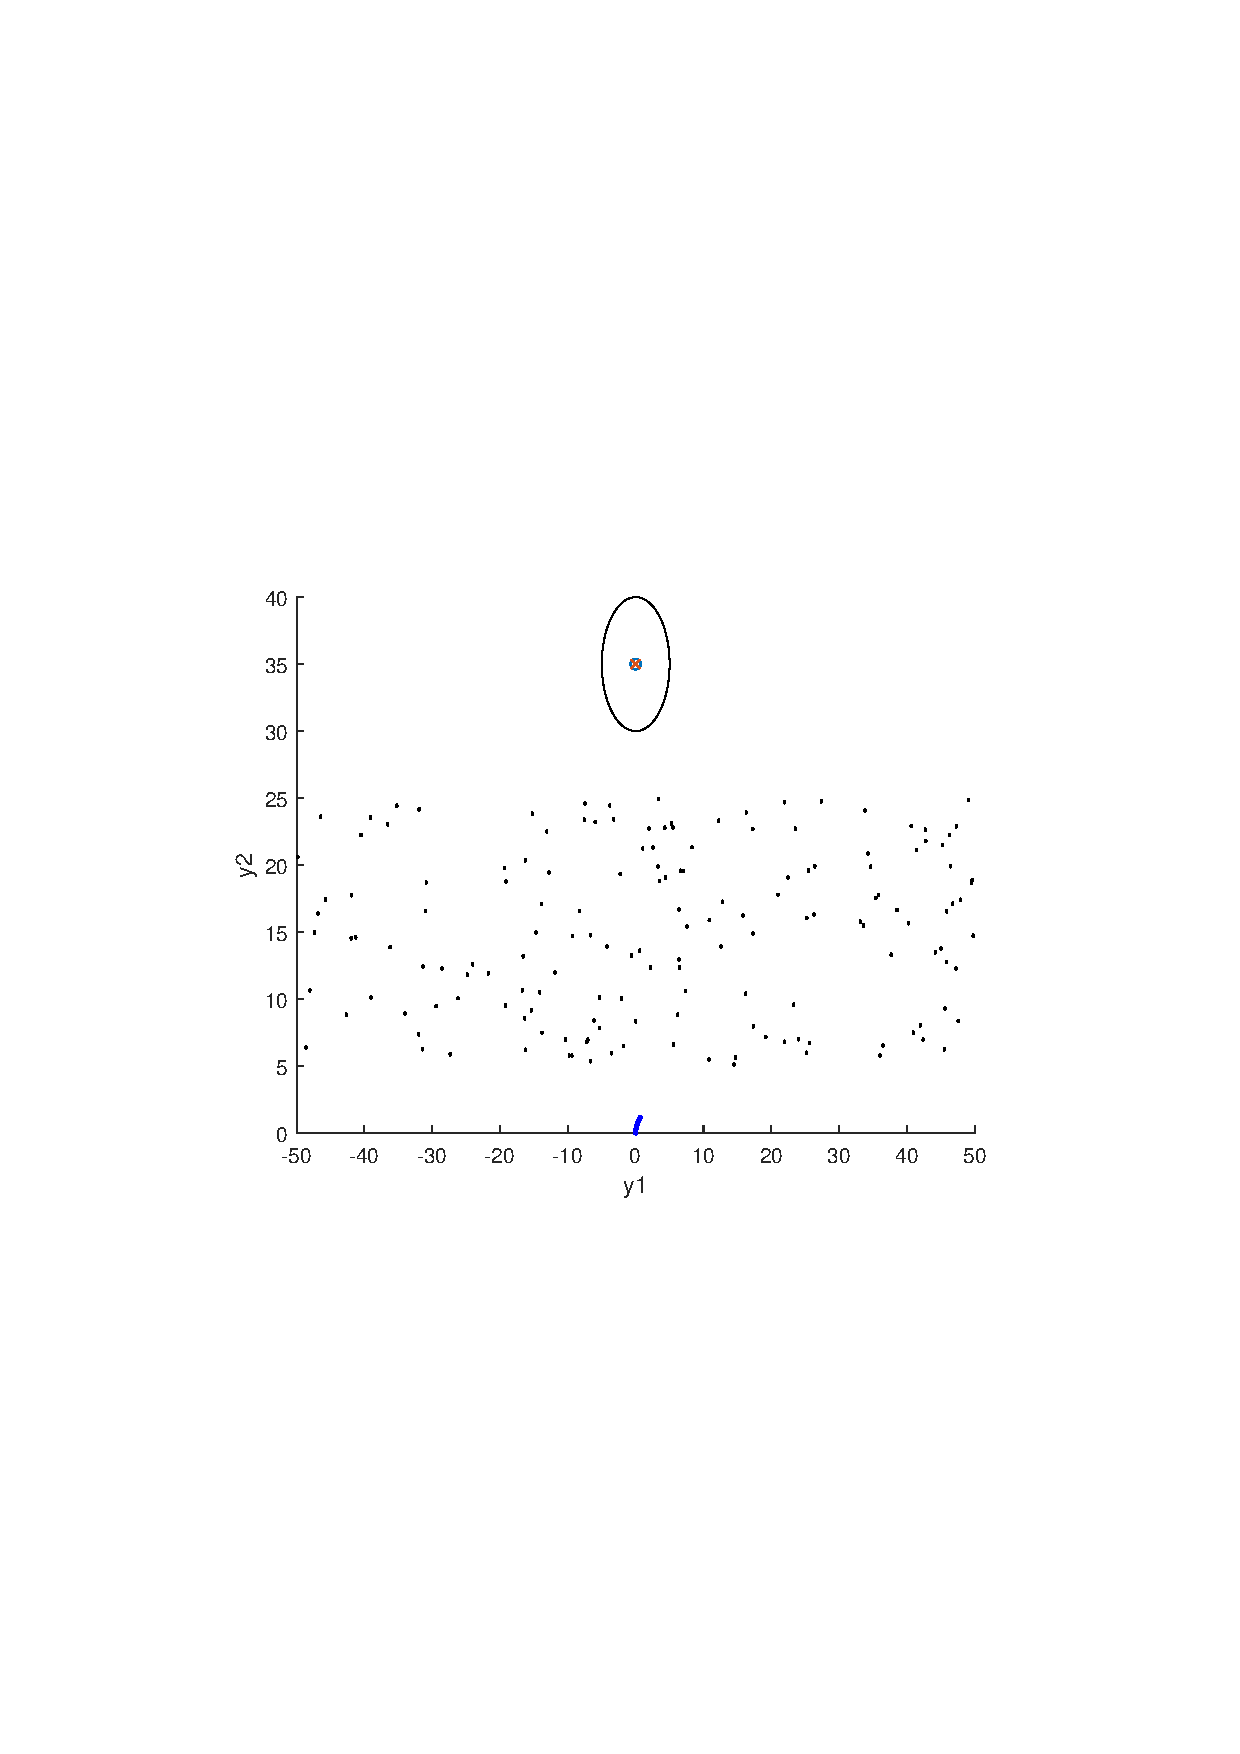
\includegraphics[width=1\columnwidth, trim={0cm, 10cm, 0cm, 9cm}, clip]{figures/experiments/rrtfunnel-1samples-dyn.pdf}
%%   \caption[The expansion of the \rrtfunnel algorithm at 1, and 101 iterations]{Visualized is the expansion of the \rrtfunnel algorithm at 1 iterations of the algorithm.}
%%   \end{minipage}
%%   \newline
%%   \begin{minipage}[c]{.8\columnwidth}
%%     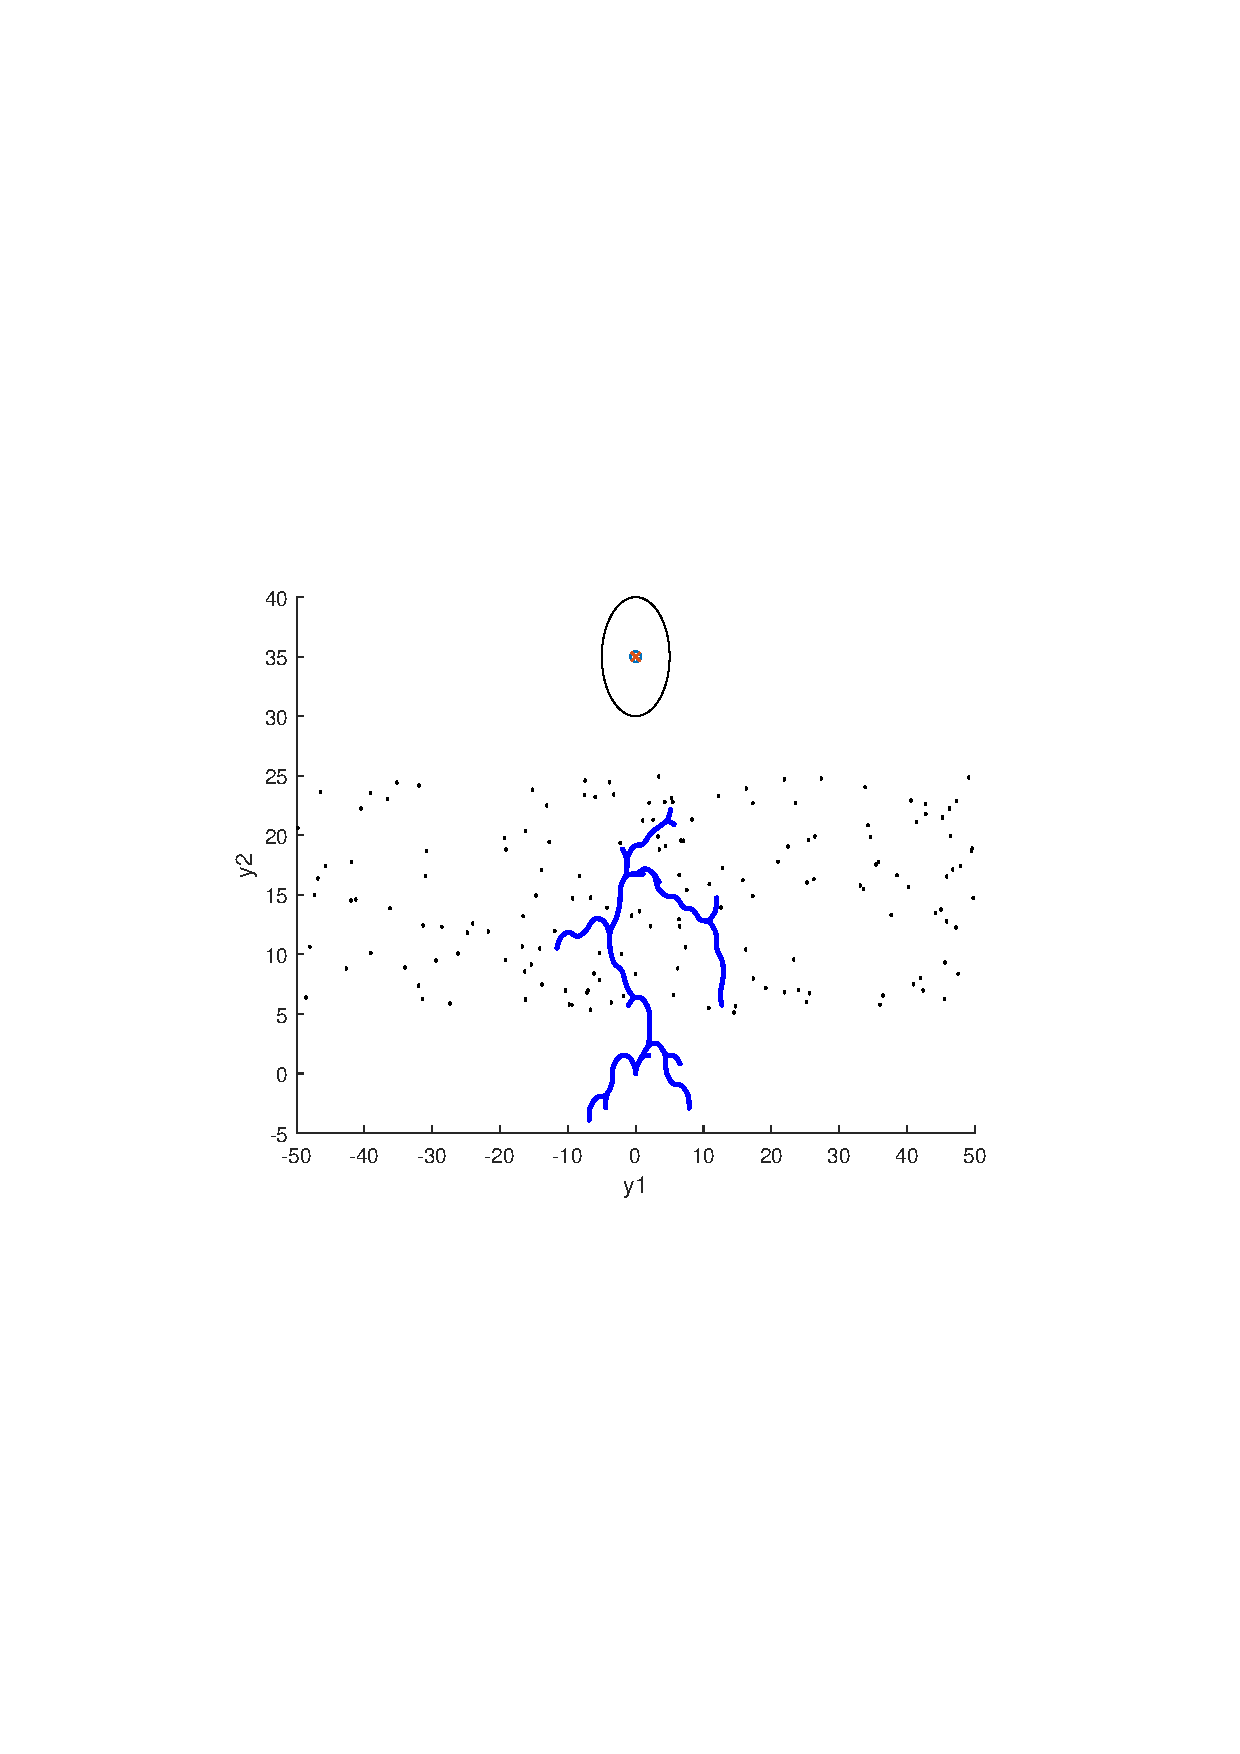
\includegraphics[width=1\columnwidth, trim={0cm, 10cm, 0cm, 9cm}, clip]{figures/experiments/rrtfunnel-101samples-dyn.pdf}
%%   \caption[The expansion of the \rrtfunnel algorithm at 1, and 101 iterations]{Visualized is the expansion of the \rrtfunnel algorithm at 101 iterations of the algorithm}
%%   \end{minipage}
%%   \newline
%%   \begin{minipage}[c]{.8\columnwidth}
%%     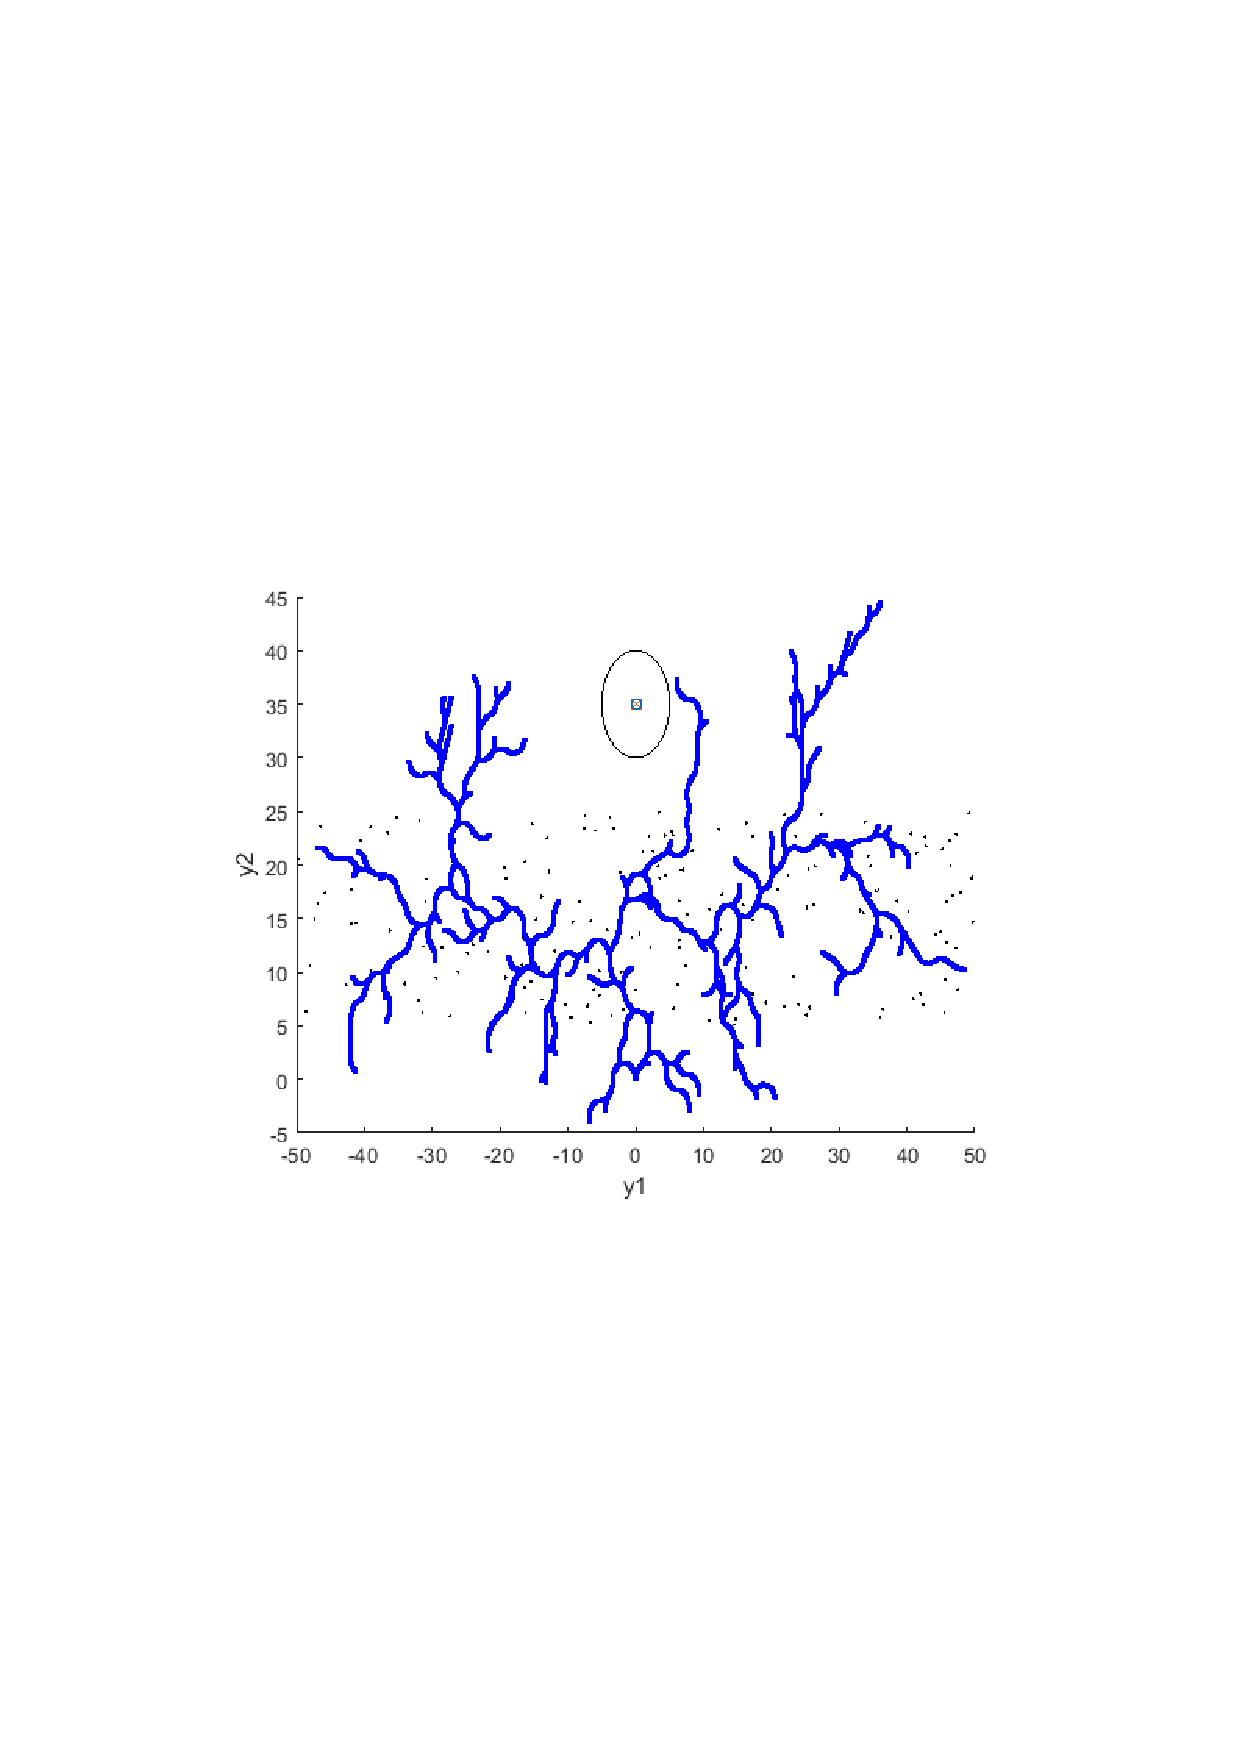
\includegraphics[width=1\columnwidth, trim={0cm, 10cm, 0cm, 9cm}, clip]{figures/experiments/rrtfunnel-701samples-dyn.pdf}
%%   \caption[The expansion of the \rrtfunnel algorithm at 1, and 101 iterations]{Visualized is the expansion of the \rrtfunnel algorithm at 701 iterations of the algorithm}
%%   \end{minipage}
%% \end{figure}

